% !TEX root =  main.tex
By Section \ref{Numerical methods for computing the Casimir energy}, to compute the Casimir energy, it is necessary to evaluate the term
$\log\det(\mathsf{V}(\mathrm{i}k)\tilde{\mathsf{V}}(\mathrm{i}k)^{-1})$ 
with different values of $k$. In this section, several efficient methods will be introduced to compute this log determinant.

The log determinant of the matrix $\mathsf{V}(\mathrm{i}k)\tilde{\mathsf{V}}(\mathrm{i}k)^{-1}$ is equal to the sum of the logarithm of the eigenvalues of 
$\mathsf{V}(\mathrm{i}k)\tilde{\mathsf{V}}(\mathrm{i}k)^{-1}$. Since $\tilde{\mathsf{V}}(\mathrm{i}k)$ is a compact perturbation of $\mathsf{V}(\mathrm{i}k)$,
most of the eigenvalues of the matrix $\mathsf{V}(\mathrm{i}k)\tilde{\mathsf{V}}(\mathrm{i}k)^{-1}$ are close to 1 
(shown in Figure \ref{eigenvalues of VVtilde}) and contribute little to the value of the Casimir energy. Hence, we do not need to compute all eigenvalues but only
the extremal ones, making subspace methods such as Krylov solvers attractive for this problem.

\begin{figure}[H]
    \centering
    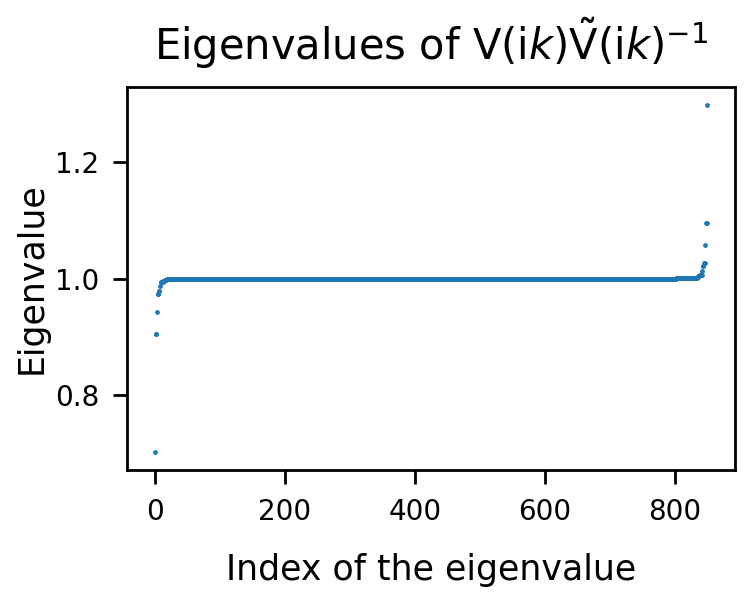
\includegraphics[scale = 0.5]{figures/Scalar_eigenvalues_around_1.png}
    \caption{The eigenvalues of the matrix $\mathsf{V}(\mathrm{i}k)\tilde{\mathsf{V}}(\mathrm{i}k)^{-1}$ when $\mathrm{i}k = 0.8\mathrm{i}$.
    The scatterers are two spheres with equal radii $r_{1} = r_{2} = 1$ and the minimal distance between them is $Z = 0.5$. The grid size of the mesh is $h = 0.2$.}
    \label{eigenvalues of VVtilde}
\end{figure}

In what follows we demonstrate and compare iterative solver approaches based on standard Arnoldi iterations \cite{arnoldi1951principle, MR3396212}, and based on the 
inverse free Krylov subspace method \cite{golub2002inverse, money2005algorithm}.
We will also discuss on acceleration strategy which is based on the idea of recycling projection bases from one quadrature point to the next. 
\subsection{Method I: Standard Arnoldi method}
The first efficient method for solving our eigenvalue problem $\mathsf{V}(\mathrm{i}k)\tilde{\mathsf{V}}(\mathrm{i}k)^{-1}\boldsymbol{x} = \lambda\boldsymbol{x}$ 
is the Arnoldi method \cite[Section 6.2]{MR3396212}. The idea of this method is to use Arnoldi iterations to construct the Krylov subspace  
$K_{m}(\mathsf{V}(\mathrm{i}k)\tilde{\mathsf{V}}(\mathrm{i}k)^{-1}, \boldsymbol{b})$, where $\boldsymbol{b}$ is some 
initial vector and $m$ is the dimension of this Krylov subspace, and to then compute the eigenvalues of the resulting projected Hessenberg matrix $H_m$ (see \cite{saad2011numerical}).
These eigenvalues have a good approximation on the extreme eigenvalues of $\mathsf{V}(\mathrm{i}k)\tilde{\mathsf{V}}(\mathrm{i}k)^{-1}$ \cite[Proposition 6.10, Theorem 6.8]{MR3396212}. 

The main cost of this standard Arnoldi method is the computation of the Krylov subspace $K_{m}$. In this process, one has to compute the matrix-vector product 
$\tilde{\mathsf{V}}^{-1}\boldsymbol{y}$, for some vector $\boldsymbol{y}$, which is equivalent to solve the linear system $\tilde{\mathsf{V}}\boldsymbol{x} = \boldsymbol{y}$. This can be 
efficiently implemented as the matrix $\tilde{\mathsf{V}}$ is a block diagonal matrix. Therefore, we just need to compute the LU decomposition for each diagonal 
block, $\mathsf{V}_{jj}$ rather than the whole system matrix and apply the forward and backward substitution to solve the linear system 
$\mathsf{V}_{jj}\,\boldsymbol{x}_j = \boldsymbol{y}_j$. Note that if all the scatterers are identical, one only needs to compute one diagonal block and one LU decomposition. 

\subsection{Method II: Inverse-free Krylov subspace method}
An alternative to the standard Arnoldi method is the inverse-free projection method, which is also based on the Arnoldi iterations but without computing any 
matrix inversions. Consider the eigenvalue problem $\mathsf{V}(\mathrm{i}k)\tilde{\mathsf{V}}(\mathrm{i}k)^{-1}\boldsymbol{x} = \lambda\boldsymbol{x}$,
it is equivalent to the following generalized eigenvalue problem:
\begin{align}\label{GEP}
    \mathsf{V}(\mathrm{i}k)\tilde{\boldsymbol{x}} = \lambda \tilde{\mathsf{V}}(\mathrm{i}k)\tilde{\boldsymbol{x}}.
\end{align}

An important property of this problem is that as we are only interested in $\mathrm{i}k$ along the imaginary axis, the corresponding matrix $\tilde{\mathrm{V}}(\mathrm{i}k)$ is positive definite,
and $\mathrm{V}(\mathrm{i}k)$ is still symmetric.

In \cite{golub2002inverse, money2005algorithm},
the authors proposed an inverse-free Krylov subspace method for computing a few extreme eigenvalues of the symmetric definite generalized eigenvalue problem.
The following algorithm summarizes the method.

\begin{algorithm}[H]
    \SetAlgoLined
    Input: Symmetric matrix $A\in\mathbb{R}^{n\times n}$, s.p.d matrix $B\in\mathbb{R}^{n\times n}$, an initial approximation $\boldsymbol{x}$ with $||\boldsymbol{x}|| = 1$,
    a given shift $\rho$ and the dimension of the Krylov subspace $m\geq 1$\\
    Output: A set of approximate eigenvalues of $A\boldsymbol{x} = \lambda B\boldsymbol{x}$ and associated eigenvectors.\\
    \begin{algorithmic}[1]
        
        \STATE Construct a basis $Z_{m}$ for the Krylov subspace $K_{m} = \text{span}(\boldsymbol{x}, (A - \rho B)\boldsymbol{x}, \dots, (A - \rho B)^{m-1}\boldsymbol{x})$ with dimension $m$
        \STATE Project $A$ and $B$ on $Z$: $A_{m} = Z_{m}^{T}(A - \rho B)Z_{m}$, $B_{m} = Z_{m}^{T}BZ_{m}$
        \STATE Compute all the eigenpairs $\{(\tilde{\lambda}_{i}, \boldsymbol{x}_{i})\}_{i = 1, \dots, m}$ for the matrix pencil $(A_{m}, B_{m})$
        \STATE Reverse the shift to obtain $\lambda_{i} = \tilde{\lambda}_{i} + \rho$.
        \end{algorithmic}
    \caption{Inverse-free Krylov subspace method for computing multiple extreme eigenvalues of the generalized eigenvalue problem $A\boldsymbol{x} = \lambda B\boldsymbol{x}$}
    \label{Alg for computing the evals kry}
    \end{algorithm}
   
    
% {\color{red} Why do you say extreme? Isn't the algorithm finding eigenvalues close to the shift?} 
Algorithm \ref{Alg for computing the evals kry} approximates $m$ eigenvalues close to the shift $\rho$ 
for the matrix pencil $(A,B)$, where $m$ is the dimension of the 
Krylov subspace $K_{m}$ in Step 1, Algorithm \ref{Alg for computing the evals kry}. The question is what shift strategy to use for $\rho$. In numerical experiments it turned
out that for the KSSF problem choosing $\rho=1$ sufficiently approximate the eigenvalues that have the main contribution to $\log\det(\mathsf{V}(\mathrm{i}k_{j})\tilde{\mathsf{V}}(\mathrm{i}k_{j})^{-1}) $.
Additionally, the main cost of this inverse free Krylov subspace method is the computation of the Krylov subspace and the projection of the matrices $A$ and $B$. In our case these are large dense matrices representing
integral operators. 
% The dominant cost of the inverse-free Krylov subspace method is that of the involved matrix-vector products with the integral operators in the process of the
% computation of the Krylov subspace $K_m$ and the projection of the shifted matrix $(A−\rho B)$ and $B$ onto the orthogonal basis of $K_m$.

\subsection{Recycling Krylov subspace based variant}

The main cost of the standard Arnoldi method and inverse-free method comes from the matrix-vector products (matvecs) in the Arnoldi iterations, where the 
involving matrices are large and dense as they represent discretized integral operators. In order to reduce the computational cost of a Krylov subspace basis 
for each wavenumber $\mathrm{i}k$, we introduce a subspace recycling based method for speeding up the computational process. This can be regarded 
as a variant of these two methods.

This recycling strategy is based on the idea that a Krylov subspace for a previous quadrature
point in the KSSF integral will be a good approximation to a Krylov subspace for the current quadrature point. We initially compute a Krylov basis for the wavenumber $\mathrm{i}k_{1}$ associated with the first
quadrature point. We then extract several eigenvectors associated with the extremal eigenvalues based on Algorithm \ref{Alg for computing the evals kry} and then orthogonalize to obtain an initial approximation
basis for the wavenumber $\mathrm{i}k_2$. For this wavenumber we project the matrices onto the recycled basis, compute approximate eigenpairs $(\tilde{\lambda}_i, \tilde{\mathbf{x}}_i)$ and then extend the subspace
basis with the residuals $\boldsymbol{r}_i = \mathsf{V}(\mathrm{i}k)\tilde{\boldsymbol{x}}_i - \tilde{\lambda}_i\tilde{\mathsf{V}}(\mathrm{i}k)\tilde{\boldsymbol{x}}_i$. With the extended subspace we recompute the eigenpairs for the second wavenumber's
case and extract eigenvectors as starting basis for the third wavenumber, and so on.

\subsection{Numerical results}
In this section, we compare the performance of standard Arnoldi and inverse-free Krylov subspace method and their recycled variants on computing the log 
determinant term of $\mathsf{V}(\mathrm{i}k)\tilde{\mathsf{V}}(\mathrm{i}k)^{-1}$. As the dominant cost of these methods is the matrix-vector products (matvec) 
associated with the discretized boundary integral operators, 
we will also compare the number of the matvecs between these methods. All the tests are performed on two spheres with equal radii $r_1 = r_2 = 1$. 
The sphere meshes are refined with size $h = 0.1$ and this results in the matrix size $\mathrm{V}(\mathrm{i}k)$ being $3192\times 3192$. Again, the minimum distance between them is denoted by $Z$, which is set as 0.5, 1.5 and 3.0. 
The number of the quadrature points is 20.

We start by comparing the relative error for approximating the $\log\det\mathsf{V}(\mathrm{i}k)\tilde{\mathsf{V}}(\mathrm{i}k)^{-1}$ using all these methods. 
The dimension of the Krylov subspace $K_m$ in all the algorithms is $m = 100$. 
For the methods with subspace recycled, the number of the recycled eigenvectors is not fixed but depends on the number of the relevant eigenvalues in each wavenumber case. 
In our experiments, we only recycle the eigenvector whose corresponding eigenvalue has the logarithm value greater than $10^{-s}$, where $s = 3, 4, 5$ when $Z = 0.5$, 1.5, 3.0, respectively, in which case the estimates of the log determinant have at least three significant digits match with the ones obtained from the direct computations. With these settings, the number of the recycled
eigenvectors becomes less and less as the $k$ gets larger.  Figure \ref{Dimension_of_the_extended_subspace} plots the dimension of the extended subspace
for each wavenumber case. It is equal to the number of the recycled eigenvectors plus the number of the residuals $\{\mathbf{r}_{i}\}_{i}$.


\begin{figure}[H]
    \centering
    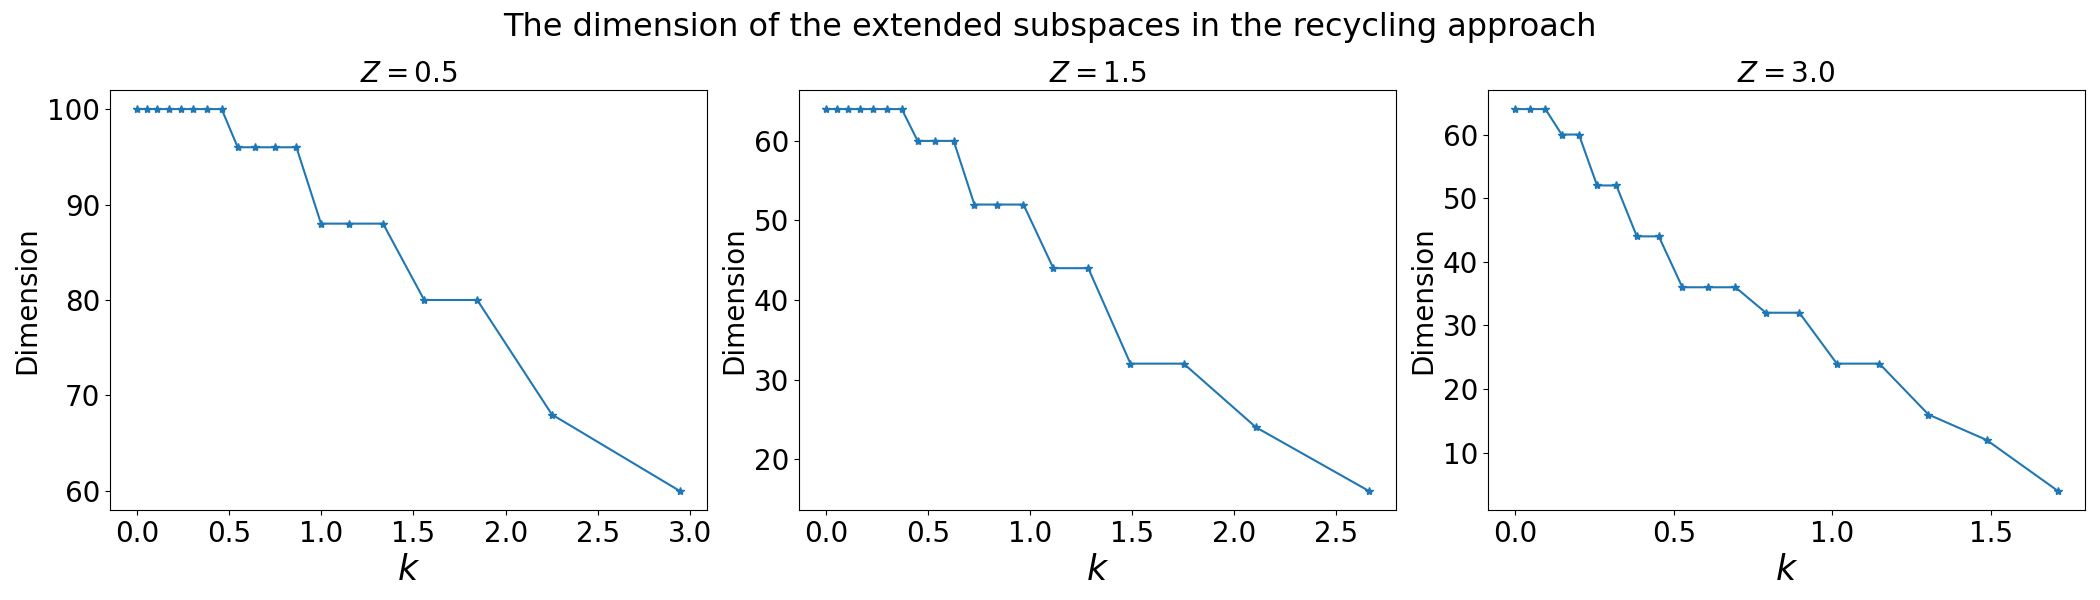
\includegraphics[width = \textwidth]{figures/Dimension_of_the_extended_subspace.png}
    \caption[Caption for LOF]{The dimension of the extended subspace in the inverse-free Krylov subspace\protect\footnotemark with subspace recycled for each $k$ in $\log\det(\mathsf{V}(\mathrm{i}k)\tilde{\mathsf{V}}(\mathrm{i}k)^{-1})$, which is equal to the number of the recycled 
    eigenvectors plus the number of the residuals $\{\mathbf{r}_{i}\}_{i}$. The recycled eigenvector has the corresponding eigenvalue whose logarithm
    is larger than $10^{-s}$, where $s = 3, 4, 5$ when $Z = 0.5, 1.5, 3.0$, respectively.}
    \label{Dimension_of_the_extended_subspace}
\end{figure}
\footnotetext{Same figure also applies for standard Arnoldi methods.}

Table \ref{Table lists the logdet} lists the relative error for approximating the value of $\log\det(\mathsf{V}(\mathrm{i}k)\tilde{\mathsf{V}}(\mathrm{i}k)^{-1})$ 
computed via the inverse-free Krylov subspace method and standard Arnoldi method with or without recycling the subspace. The reference value is computed by the 
direct dense computation of the log determinant. The wavenumbers $\mathrm{i}k$ are chosen to be associated with the first five consecutive quadrature points, 
whose corresponding log determinant values account for a great proportion in the Casimir integral. 

This table indicates that with the settings above, one can have at least three significant digits accuracy and the accuracy of the methods with subspace 
recycled is similar to the ones without any recycling processes. As for the performance of these methods and their variants at larger quadrature points, we 
cannot always have three digits accuracy. However, this will not affect the estimates of the Casimir energy too 
much as their corresponding log determinant value is relatively smaller than the others and contributes very little to the Casimir energy. 
 
\begin{table}[H]
    \centering
    \begin{tabular}{ |M{1.5cm}|M{2.0cm}|M{2.2cm} |M{2.2cm}|M{3cm}|M{3cm}|M{2.2cm}| } 
    \hline
    Distance $Z$ & Wavenumber $k$ &  Inverse-free (no recycling) & Inverse-free (recycling) & Standard Arnoldi (no recycling) & Standard Arnoldi (recycling)\\
    \hline
    \multirow{5}{4em}{$Z = 0.5$}   & 0        & $9.79\times 10^{-4}$  & $9.79\times 10^{-4}$  &$9.29\times 10^{-4}$ &$9.29\times 10^{-4}$\\ 
                                   & 0.0540   & $9.67\times 10^{-4}$  & $9.78\times 10^{-5}$  &$4.91\times 10^{-5}$ &$1.37\times 10^{-6}$\\ 
                                   & 0.111    & $1.22\times 10^{-3}$  & $2.79\times 10^{-5}$  &$5.29\times 10^{-5}$ &$5.17\times 10^{-6}$\\ 
                                   & 0.171    & $1.15\times 10^{-3}$  & $2.42\times 10^{-5}$  &$2.78\times 10^{-5}$ &$8.45\times 10^{-5}$\\ 
                                   & 0.236    & $1.25\times 10^{-3}$  & $9.10\times 10^{-6}$  &$1.12\times 10^{-4}$ &$2.76\times 10^{-5}$\\ 
    \hline
    \hline
    \multirow{5}{4em}{$Z = 1.5$}   & 0        & $9.48\times 10^{-4}$  & $9.54\times 10^{-4}$  &$3.41\times 10^{-7}$ &$3.41\times 10^{-7}$\\ 
                                   & 0.0530   & $1.02\times 10^{-3}$  & $2.87\times 10^{-4}$  &$5.89\times 10^{-7}$ &$3.97\times 10^{-8}$\\ 
                                   & 0.109    & $1.16\times 10^{-3}$  & $1.80\times 10^{-4}$  &$1.45\times 10^{-8}$ &$2.35\times 10^{-4}$\\ 
                                   & 0.168    & $1.25\times 10^{-3}$  & $1.35\times 10^{-4}$  &$2.70\times 10^{-6}$ &$1.06\times 10^{-4}$\\ 
                                   & 0.231    & $1.33\times 10^{-3}$  & $4.77\times 10^{-5}$  &$3.14\times 10^{-7}$ &$4.87\times 10^{-5}$\\ 
    \hline
    \hline
    \multirow{5}{4em}{$Z = 3.0$}   & 0        & $1.38\times 10^{-3}$  & $1.38\times 10^{-3}$  &$8.55\times 10^{-12}$ &$8.55\times 10^{-12}$\\ 
                                   & 0.0465   & $1.54\times 10^{-3}$  & $4.34\times 10^{-4}$  &$3.46\times 10^{-9}$  &$2.61\times 10^{-5}$\\ 
                                   & 0.0954   & $1.81\times 10^{-3}$  & $2.89\times 10^{-4}$  &$5.02\times 10^{-10}$ &$5.43\times 10^{-7}$\\ 
                                   & 0.146    & $2.13\times 10^{-3}$  & $2.35\times 10^{-4}$  &$4.82\times 10^{-8}$  &$2.50\times 10^{-5}$\\ 
                                   & 0.200    & $2.54\times 10^{-3}$  & $2.13\times 10^{-4}$  &$5.07\times 10^{-9}$  &$1.59\times 10^{-5}$\\ 
    \hline
    \end{tabular}
    \caption{Relative error for approximating the value of $\log\det(\mathrm{V}(\mathrm{i}k)\tilde{\mathrm{V}}(\mathrm{i}k)^{-1})$ on the wavenumbers associated with the first five consecutive 
    quadrature points via the inverse-free Krylov subspace and standard Arnoldi methods with/without subspace recycled. The shift is set as $\rho = 1$ for the inverse-free method. The recycled eigenvector has the corresponding eigenvalue whose logarithm
    is larger than $10^{-s}$, where $s = 3, 4, 5$ when $Z = 0.5, 1.5, 3.0$, respectively.}
    \label{Table lists the logdet}
    \end{table}
    
    Recall that the main cost in these algorithms is from the computation of the Krylov basis and the matrix projections. For large problems, 
    the dominating cost is the involved matrix-vector products with the discretized integral operators. We count the number of matvecs associated with the 
    discretized integral operators ($\mathsf{V}_{ij}$) for each algorithm and the results are summarized in Table \ref{4methods_matvecs}.


    \begin{table}[H]
        \centering
    
    \begin{tabular}{ |P{3cm}|P{3.8cm}|P{3cm}|P{3.6cm}|}
    
        \hline
        \multicolumn{2}{|c|}{Inverse-free Krylov subspace method}& \multicolumn{2}{c|}{Standard Arnoldi method} \\
        \hline
      Without recycling &  With recycling & Without recycling& With recycling\\
        \hline
        $(6m - 2)N_q$  & $(6m - 2) + 12\sum\limits_{i = 1}^{N_q-1}s_{i}$   & $(4m - 4)N_q$ &   $(4m - 4) + 8\sum\limits_{i = 1}^{N_q-1}s_{i}$ \\
        \hline
      \end{tabular}
      \bigskip
      \caption{The number of matvecs associated with the discretized integral operators inside the inverse-free Krylov subspace and standard Arnoldi methods with or without recycling subspace.
      $N_q$ is the number of wavenumbers/quadrature points, $m$ is the dimension of the Krylov subspace for the first wavenumber (in recycling case); for all the wavenumbers (in non-recycling case),
      and $s_{i}$ is the number of the recycled eigenvectors 
      from the $i$th wavenumber's case (in recycling case)}
      \label{4methods_matvecs}
    \end{table}


    In Figure \ref{fig:Num_matvec}, we plot the number of actual matvecs associated with the discretized matrix form $\mathsf{V}_{ij}$, for $i, j = 1, 2, \cdots, N$ in each individual algorithm when computing the Casimir energy between 2 spheres with different different distance $Z$. It shows that the recycling strategy significantly reduces the overall number of matvecs. Although the number of matvecs in standard Arnoldi method with subspace recycled (light red in Figure \ref{fig:Num_matvec}) is smaller than the one of the inverse-free method  with subspace recycled (light blue in Figure \ref{fig:Num_matvec}), one has to compute the LU decomposition for each diagonal block in each Arnoldi iteration, which has cubic complexity. 

    \begin{figure}[H]
        \centering
        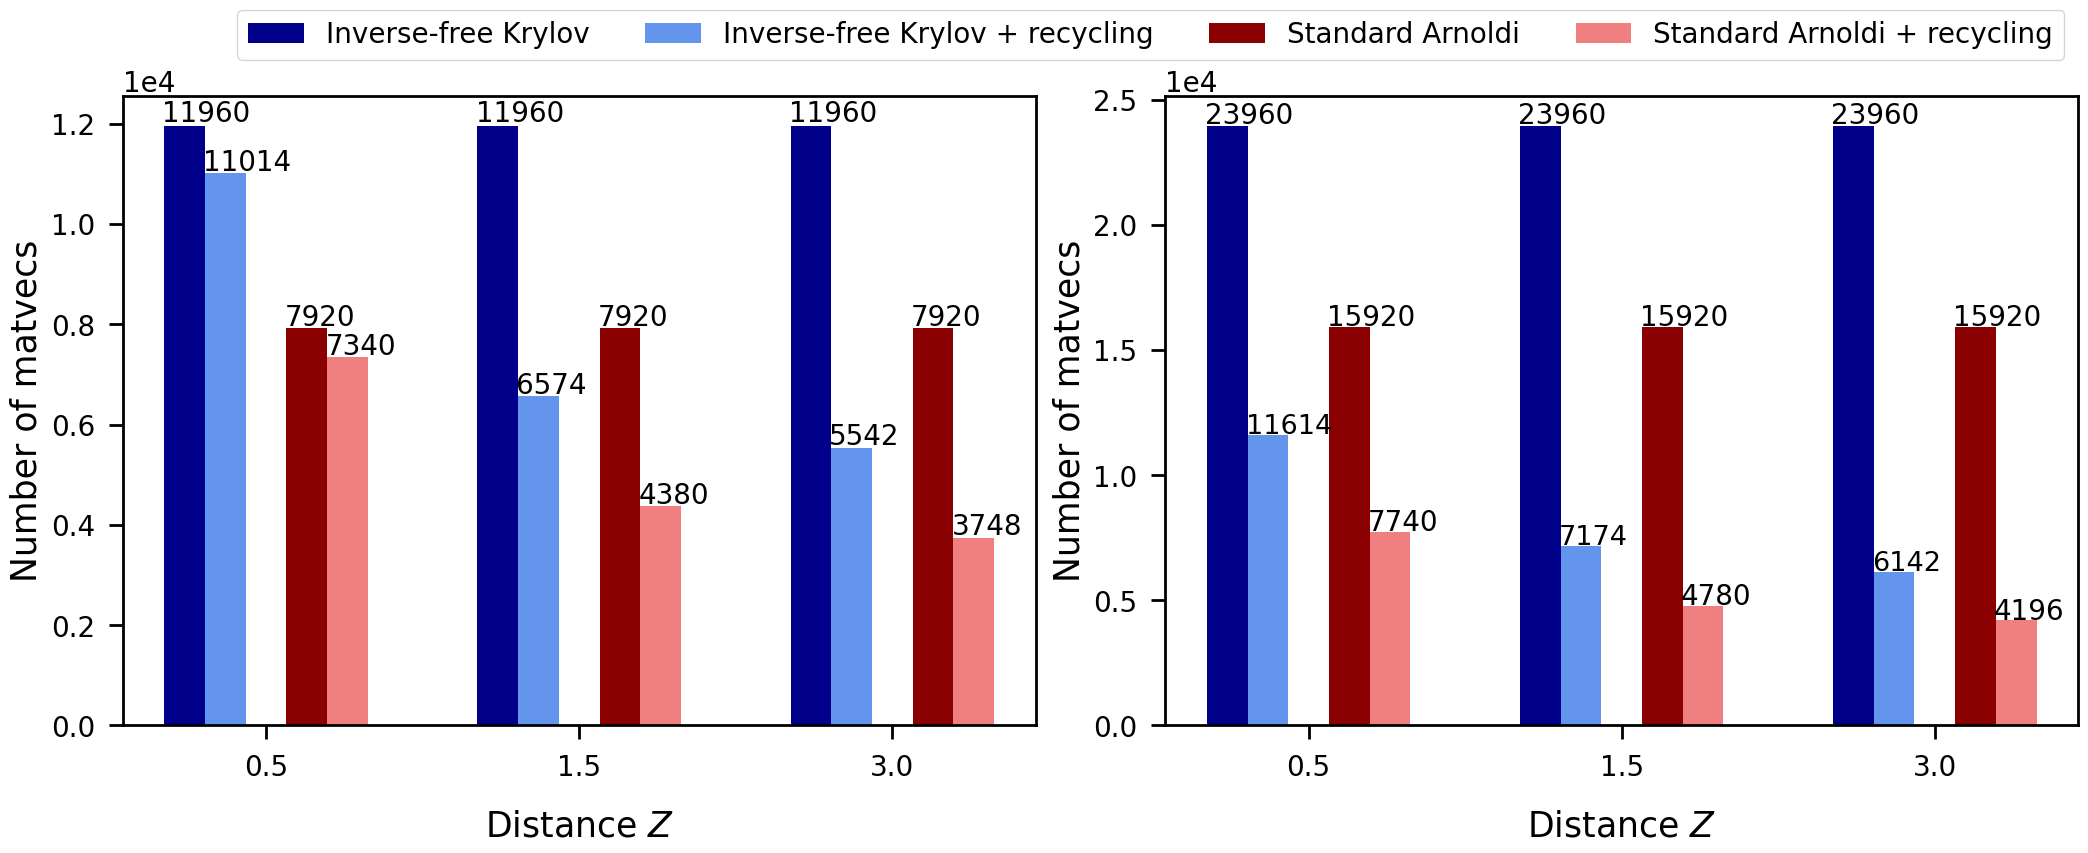
\includegraphics[width = \textwidth]{figures/Num_matvec.png}
        \caption{The number of matvecs inside the inverse-free and standard Arnoldi methods with or without recycling subspace when 
        computing the normalized Casimir energy between two spheres with equal radii $R = 1$ and the distance $Z$ is 0.5, 1.5 and 3.0. 
        The number of the quadrature point is $N_q = 20$. The dimension of the Krylov subspace is set as $m = 100$ ({\color{gray} Left}) and 
        $200$ ({\color{gray} Right}).}
        \label{fig:Num_matvec}
    \end{figure}

%Note that for the recycled methods Algorithm \ref{Alg for computing the evals kry recycled}-\ref{Alg for computing the evals arno recycled}
%we apply different rules for extracting the eigenvectors. For  
%is different which depends on the 

%For the standard Arnoldi method,  it can be noticed that the number of FLOP is cubicly increasing with the size of the matrix 
%no matter the subspace is recycled or not. For the inverse-free Krylov subspace methods, as the wavenumber $k$ increases, the number of the extreme eigenvalues
%decreases which makes the number of extracted eigenvectors decreases as well. Therefore, for the large-scale problems, the inverse-free Krylov subspace method with 
%subspaces recycled would be applied to compute the Casimir energy with lower complexity and desired accuracy.
